\section{Basic Zombie Model Introduction}

The basic SZR (susceptible-zombie-removed) model is a modification of the classical SIR model [1] which was first introduced in [17]. This model considers zombie infection as the cause of the epidemic. \\

Like the SIR model, this SZR model also categorizes the whole population into three compartments. It begins with the susceptible compartment denoted by S, then the compartment for the infected and infectious zombies Z and finally the compartment R for the removed population. \\

\begin{itemize}
	\item The susceptible compartment S, denotes the group of the population who are healthy but are vulnerable to the zombie infection. \\
	
	\item The zombie compartment Z, denotes the group of the population who are infected with zombie infection and are also infectious. This group of people are capable to spread the disease.\\
	
	\item Finally, the people who have recovered from the zombie disease are categorized in the removed R compartment.
\end{itemize}

The whole model can be visualized as below--- \\

\begin{figure}[H]
\centering
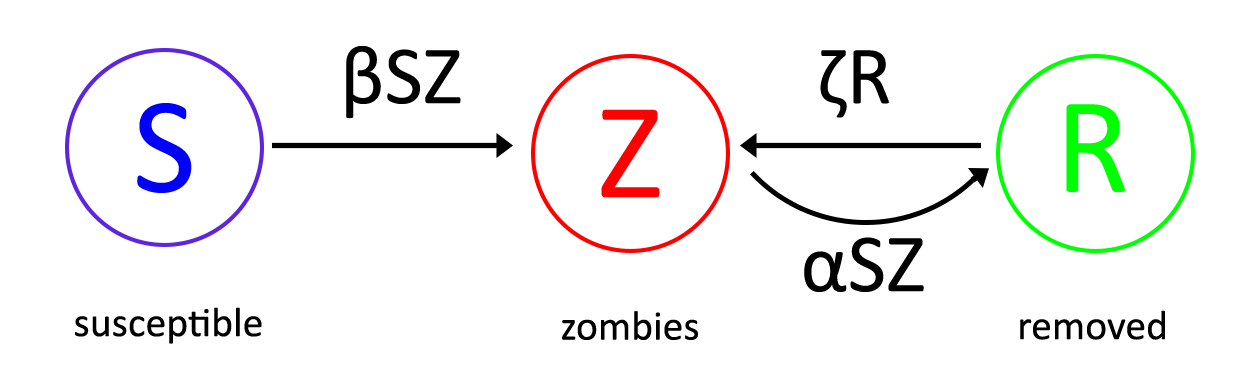
\includegraphics[scale=1.2]{SZR.png}
\caption{Basic SZR Model}
\label{fig:Basic SZR Model}
\end{figure}

The dynamics of the spread of disease within this model can be summarized as below--- 

\begin{itemize}
	\item Individuals from the susceptible compartment S transfer to the compartment of zombies Z at a rate of \textbeta SZ. Here \textbeta \ is a positive constant and is the transfer rate from the compartment S to I. The transfer rate of individuals from the susceptible to the zombies depends both on the current population number of S and Z. \\
	
	\item The transfer rate of individuals from the zombies compartment Z to the removed R is defined as \textalpha SZ, where \textalpha \ is a positive constant and the removal rate from the compartment Z to R. This removal rate also depends on the total number of individuals for both of the susceptible and zombies compartments. \\
	
	\item Finally, the reinfection rate \textzeta R, that denotes the transfer of individuals from the removed compartment to the zombies compartment. This rate is assumed to be dependent only on the total number of individuals inside the R compartment.
\end{itemize}

So now, the SZR model can be written as a system of ordinary differential equations as given below--- \\

\begin{equation}
\begin{aligned}
&S^{\prime}(t)=-\beta SZ \\
&Z^{\prime}(t)=\zeta R + (\beta - \alpha)SZ \\
&R^{\prime}(t)=\alpha SZ - \zeta R \\
\end{aligned}
\end{equation}

As before, all the variables S, Z and R are functions of time, t. And the total size of the population remains constant within the given time and the sum of all the compartments is equal to the whole population size N. Which in turn means that, \\

$ N = S(t) + Z(t) + R(t)$ 
\\

Equation (3.1) can be reduced in the following form, with the following substitution $R = N - S - Z$, \\

\begin{equation}
\begin{aligned}
&S^{\prime}(t)=-\beta SZ \\
&Z^{\prime}(t)=\zeta (N - S - Z) + (\beta - \alpha)SZ \\
\end{aligned}
\end{equation}

Some important assumptions of this model--- 

\begin{itemize}
	\item Unlike the SIR model, in the SZR model, no type of immunity is promised to the individuals of the population. So the possibility of reinfection is considered here. Hence, comes the reinfection rate \textzeta R from the removed compartment to the compartment of zombies. So the removed individuals in the compartment R can be reinfected or resurrected and can be returned to the Z compartment. \\
	
	\item Here, zombies are removed only through the interaction with human population. All types of other natural causes like starvation, natural disaster or accident are ignored in this model. \\
	
	\item As soon as a susceptible individual gets infected, that person is transferred to the zombies compartment. The incubation period is negligible and can be omitted. \\
	
	\item Like the SIR model, the population is homogeneously mixed. Every individual possesses an equal probability of getting infected. 
\end{itemize}

In [17], the authors tried to analyze the linear stability of the disease free equilibrium of this model, in order to determine the possible survivability of the human species. The authors concluded that, the survival of the human race is not possible in the long run of this model and thus the disease free equilibrium is nonexistent.

\pagebreak
\section{Example of SZR Model}

To simulate the basic SZR model, an imaginary example can be considered. \\

For this example, let us consider the following values, \\

\noindent The total population size, N = 1000 \\
Initial susceptible population, S(0) = 830 \\
Initial zombie population, Z(0) = 70 \\
Initial removed population, R(0) = 100 \\
Number of days, t = 4000 \\

And for the estimates of the parameters, those values can be taken from [17], \\

\begin{table}[h!]
\centering
 \begin{tabular}{||c c c||} 
 \hline
 Parameter & Description & Estimate \\ [1.0ex] 
 \hline\hline 
 \textbeta & transmission rate for the zombie infection & 0.0095 \\ 
 \textalpha & removal rate of infected zombies & 0.005 \\
 \textzeta & reinfection or resurrection rate for removed individuals & 0.0001 \\  [1.5ex] 
 \hline
 \end{tabular}
\caption{Parameter Estimates for the Basic SZR Model}
\label{table 3.1}
\end{table}

Now it is possible to solve the system of differential equations (3.1) numerically using python with the above set of values. \\

At first, the system is numerically solved for t = 10 days, with total steps of 100, so it is easier to visualize the decrease of the susceptible population. \\

\begin{figure}[H]
\centering
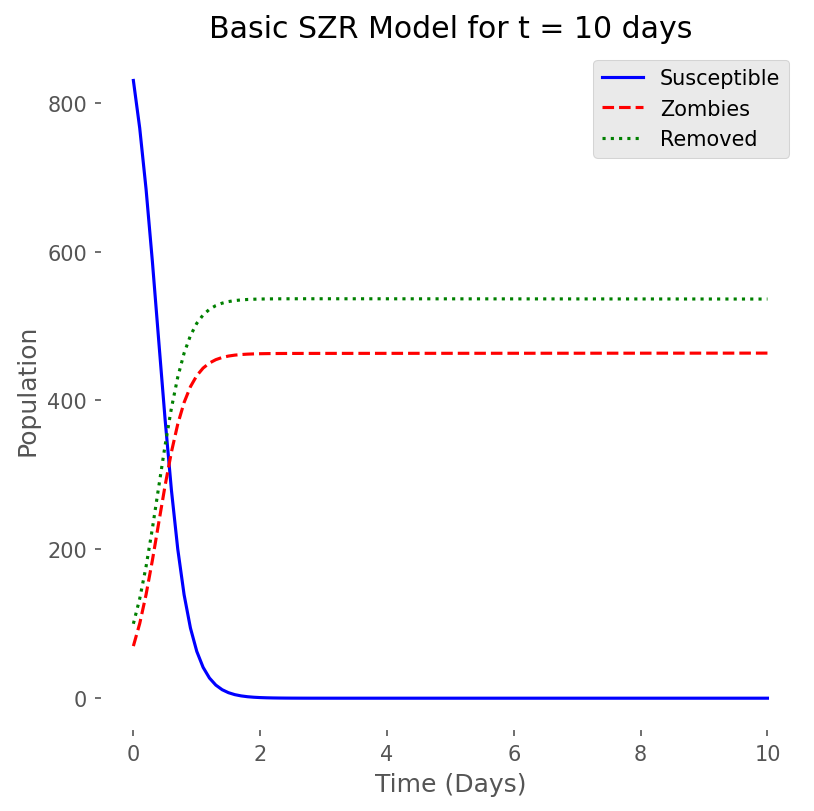
\includegraphics[scale=0.7]{SZR_10Days.png}
\caption{Basic SZR Model Numeric Solution for t = 10 Days}
\label{fig:Basic SZR 10 Days}
\end{figure}

Finally, the system is solved for t =4000 days, with total steps of 4000. As can be seen from the Figure 3.3, the number of zombies increases, while the removed population decreases on a straight manner. \\

\begin{figure}[H]
\centering
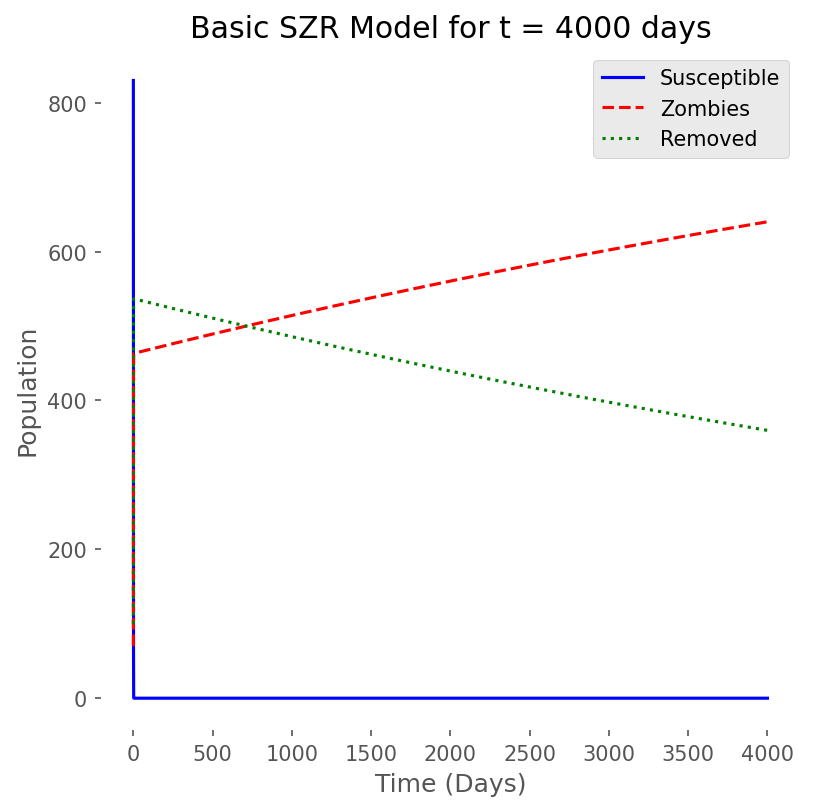
\includegraphics[scale=0.7]{SZR_4000Days.png}
\caption{Basic SZR Model Numeric Solution for t = 4000 Days}
\label{fig:Basic SZR 4000 Days}
\end{figure}

And also the phase portrait for the system--- \\

\begin{figure}[H]
\centering
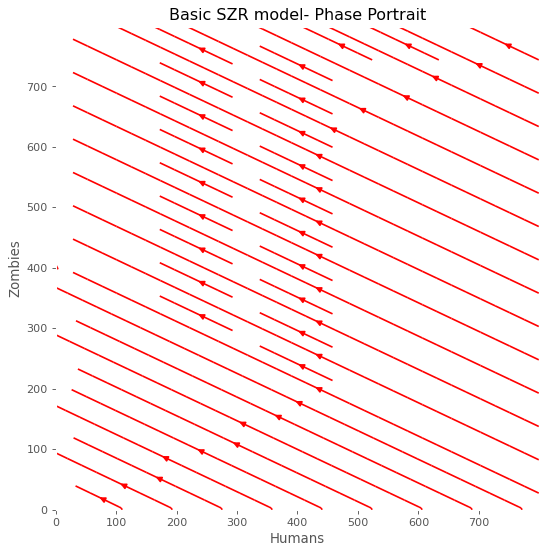
\includegraphics[scale=0.6]{SZR_PhasePortrait.png}
\caption{Basic SZR Model- Phase Portrait}
\label{fig:Basic SZR Phase Portrait}
\end{figure}

As can be seen from Figure 3.4, the phase portrait of the basic SZR model, the system is unstable and the survival of the healthy human population is not possible in this model. \\

\pagebreak
\section{SZR Model with Perturbation}
\subsection{Model Introduction}

Now comes the scope for the modification of the basic SZR model. In [18], the authors Allen et al. introduced a new parameter to perturb the basic model. \\

The authors considered a new parameter \textmu, with $\mu \in (0, \infty)$, to set up a non-linearity inside the model. Here, the removal rate from the zombies compartment Z to the removed compartment R is defined as \textalpha S\textsuperscript{(1+\textmu)}Z. \\ 

This parameter \textmu \ is introduced to slightly perturb the original basic model in order to provide rooms for new possibilities and equilibriums as well as to give it a nonlinear nature. For more methodologies on perturbation parameters, interested reader is directed to [27], [28], [29], [30], [31], [32], [33]. \\

The newly modified model can be visualized in the figure below--- \\


\begin{figure}[H]
\centering
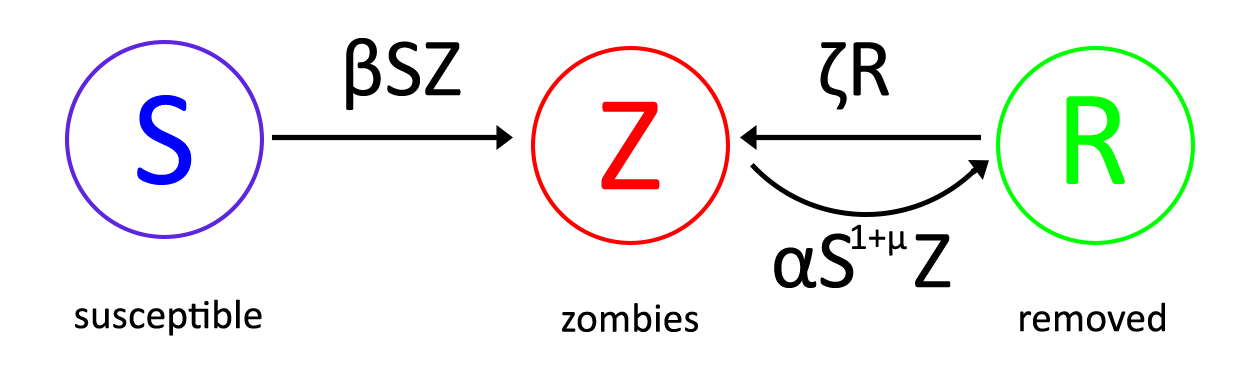
\includegraphics[scale=1.2]{SZR_mu.png}
\caption{Perturbed SZR Model}
\label{fig:Perturbed SZR Model}
\end{figure}

All the other assumptions and considerations from the basic SZR model remains same and unchanged in this modified and slightly perturbed SZR model. \\

It is expected that this small perturbation in the original SZR model will open the scope for human survival and provide a new disease free equilibrium. \\

According to this modification, a new system of differential equations can be developed--- 

\begin{equation}
\begin{aligned}
&S^{\prime}(t)=-\beta SZ \\
&Z^{\prime}(t)=\zeta R + \beta SZ - \alpha S^{1 + \mu} Z\\
&R^{\prime}(t)=\alpha S^{1 + \mu} Z - \zeta R \\
\end{aligned}
\end{equation}
\\

Or, these equations can be reduced with the substitution of $R = N - S - Z$, in the following form--- \\

\begin{equation}
\begin{aligned}
&S^{\prime}(t)=-\beta SZ \\
&Z^{\prime}(t)=\zeta (N - S - Z) + \beta SZ - \alpha S^{1 + \mu} Z\\
\end{aligned}
\end{equation}
\\

As per [18], the condition for the perturbation parameter \textmu \ to make the model linearly stable and to introduce a disease free equilibrium, is as given below---

\begin{equation}
\mu>\frac{\ln \left(\frac{\beta N-\zeta}{\alpha}\right)}{\ln (N)}-1
\end{equation}

\pagebreak
\subsection{Example}

This modified SZR model with perturbation can be numerically solved using an imaginary example, so that it is easier to understand and predict its behavior. \\

For this imaginary example, let us consider the following initial conditions--- \\

\noindent The total population size, N = 1000 \\
Initial susceptible population, S(0) = 800 \\
Initial zombie population, Z(0) = 200 \\
Initial removed population, R(0) = 0 \\
Number of days, t = 1000 \\

And for the estimates of the parameters, those values can be taken from [17] and [18], \\

\begin{table}[h!]
\centering
 \begin{tabular}{||c c c||} 
 \hline
 Parameter & Description & Estimate \\ [1.0ex] 
 \hline\hline 
 \textbeta & transmission rate for the zombie infection & 0.0095 \\ 
 \textalpha & removal rate of infected zombies & 0.005 \\
 \textzeta & reinfection or resurrection rate for removed individuals & 0.0001 \\  
 \textmu & perturbation value & 0.175 \\[1.5ex]
 \hline
 \end{tabular}
\caption{Parameter Estimates for the Perturbed SZR Model}
\label{table 3.2}
\end{table}

Now the model is solved numerically with the above set of values using Python solve\_ivp [23] function. This function uses Runge-Kutta method of order five (RK45) [61], [62], [63], as the integration method. \\

First the system is solved for 10 days, with a step size of 0.1. So, it easier to visualize the changes in the zombie population. \\

\begin{figure}[H]
\centering
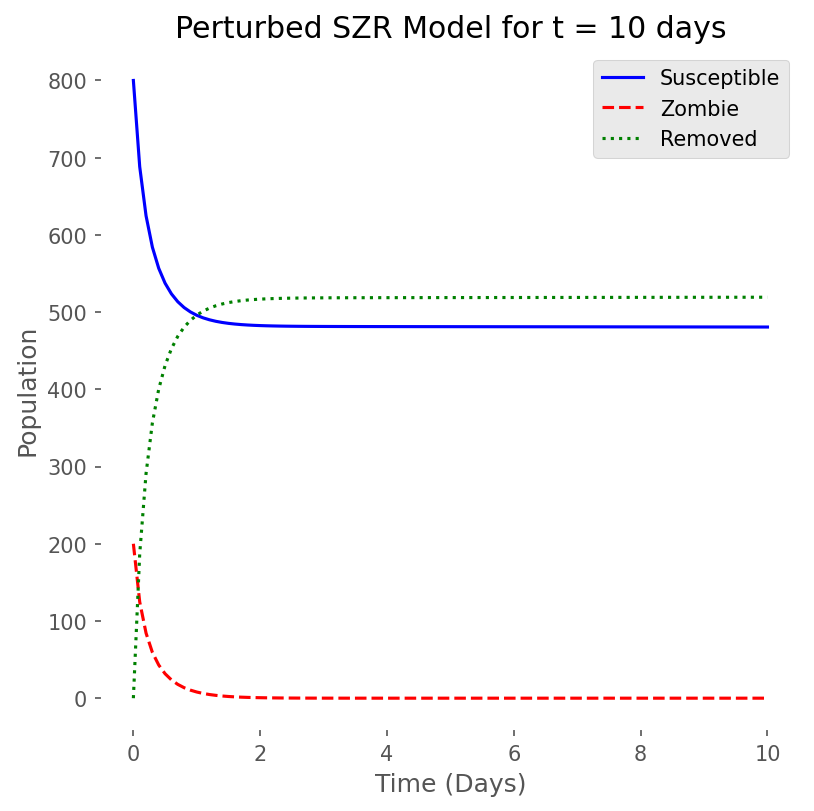
\includegraphics[scale=0.7]{PerturbedSZR_10Days_Solution.png}
\caption{Perturbed SZR Model Numeric Solution for t = 10 Days}
\label{fig:Perturbed SZR Model 10 Days}
\end{figure}

And finally, the system is solved for 1000 days, with a step size of 1. It can be seen that, the impact of the perturbation parameter \textmu \ has caused the decline of the zombie population and the size of the removed population increases gradually. \\

\begin{figure}[H]
\centering
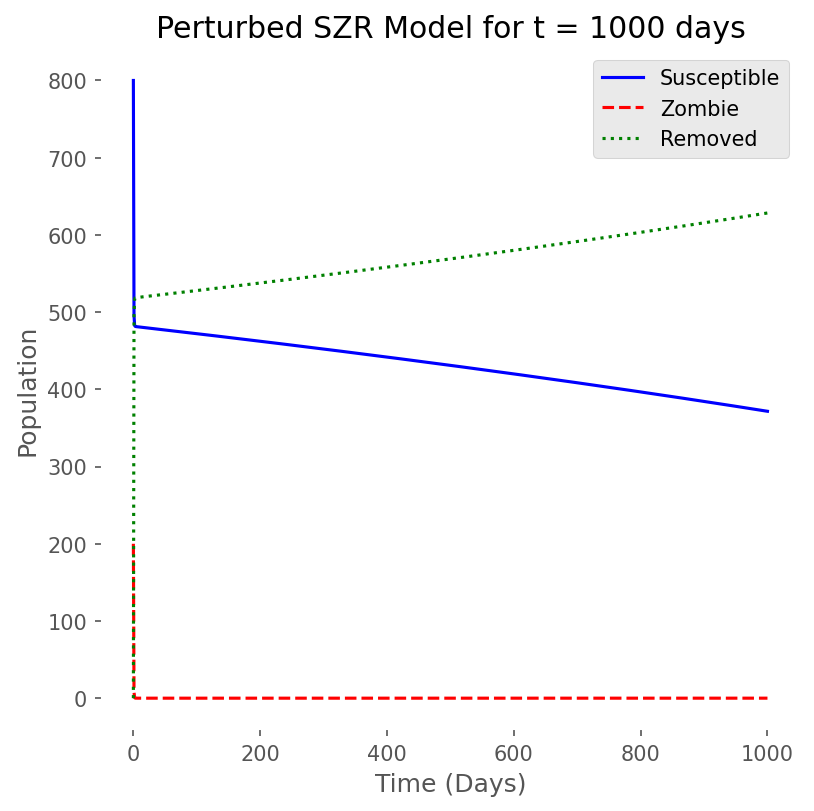
\includegraphics[scale=0.7]{PerturbedSZR_1000Days_Solution.png}
\caption{Perturbed SZR Model Numeric Solution for t = 1000 Days}
\label{fig:Perturbed SZR Model 1000 Days}
\end{figure}

Now, for the phase portrait of the perturbed SZR model, it can be seen that the perturbation parameter \textmu \ has a deep impact on the stability of the model. While comparing with the Figure 3.4, it is noticeable that this perturbation parameter has caused a noticeable change in the behavior of the model. \\

\begin{figure}[H]
\centering
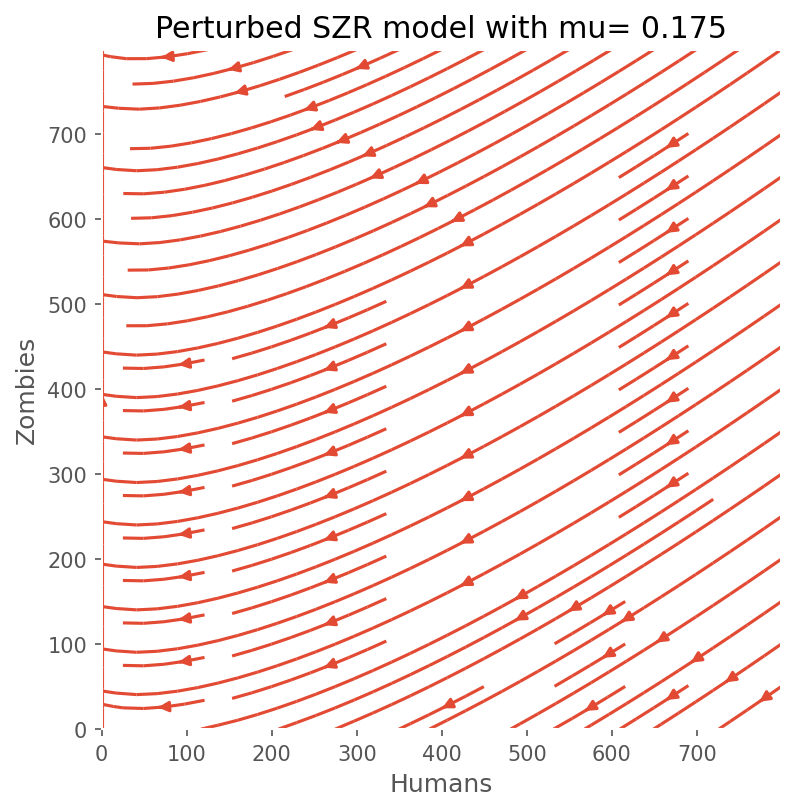
\includegraphics[scale=0.7]{PerturbedSZR_PhasePortrait_02.png}
\caption{Perturbed SZR Model- Phase Portrait}
\label{fig:Perturbed SZR Model Phase Portrait}
\end{figure}

So due to this perturbation parameter \textmu, this model is stable. The number of zombies will decrease to zero and the whole population will go back to its healthy state gradually. 

\pagebreak
\subsection{Change of Stability as Per Perturbation Parameter}

In order to investigate the change of stability and behavior of the perturbed SZR model, a simple python program was written. This program will plot the phase portraits of this model, starting from \textmu \ = 0.0 (at \textmu \ = 0.0, this model is just the basic and unperturbed SZR model), and will increase the value of \textmu \ by 0.005 at each step, until the model reaches linear stability and a disease free equilibrium exists. The value of \textmu \ is checked against the condition stated in equation (3.5), to find the first value of \textmu \ corresponding to the stability of the model. \\

\begin{figure}[H]
\centering
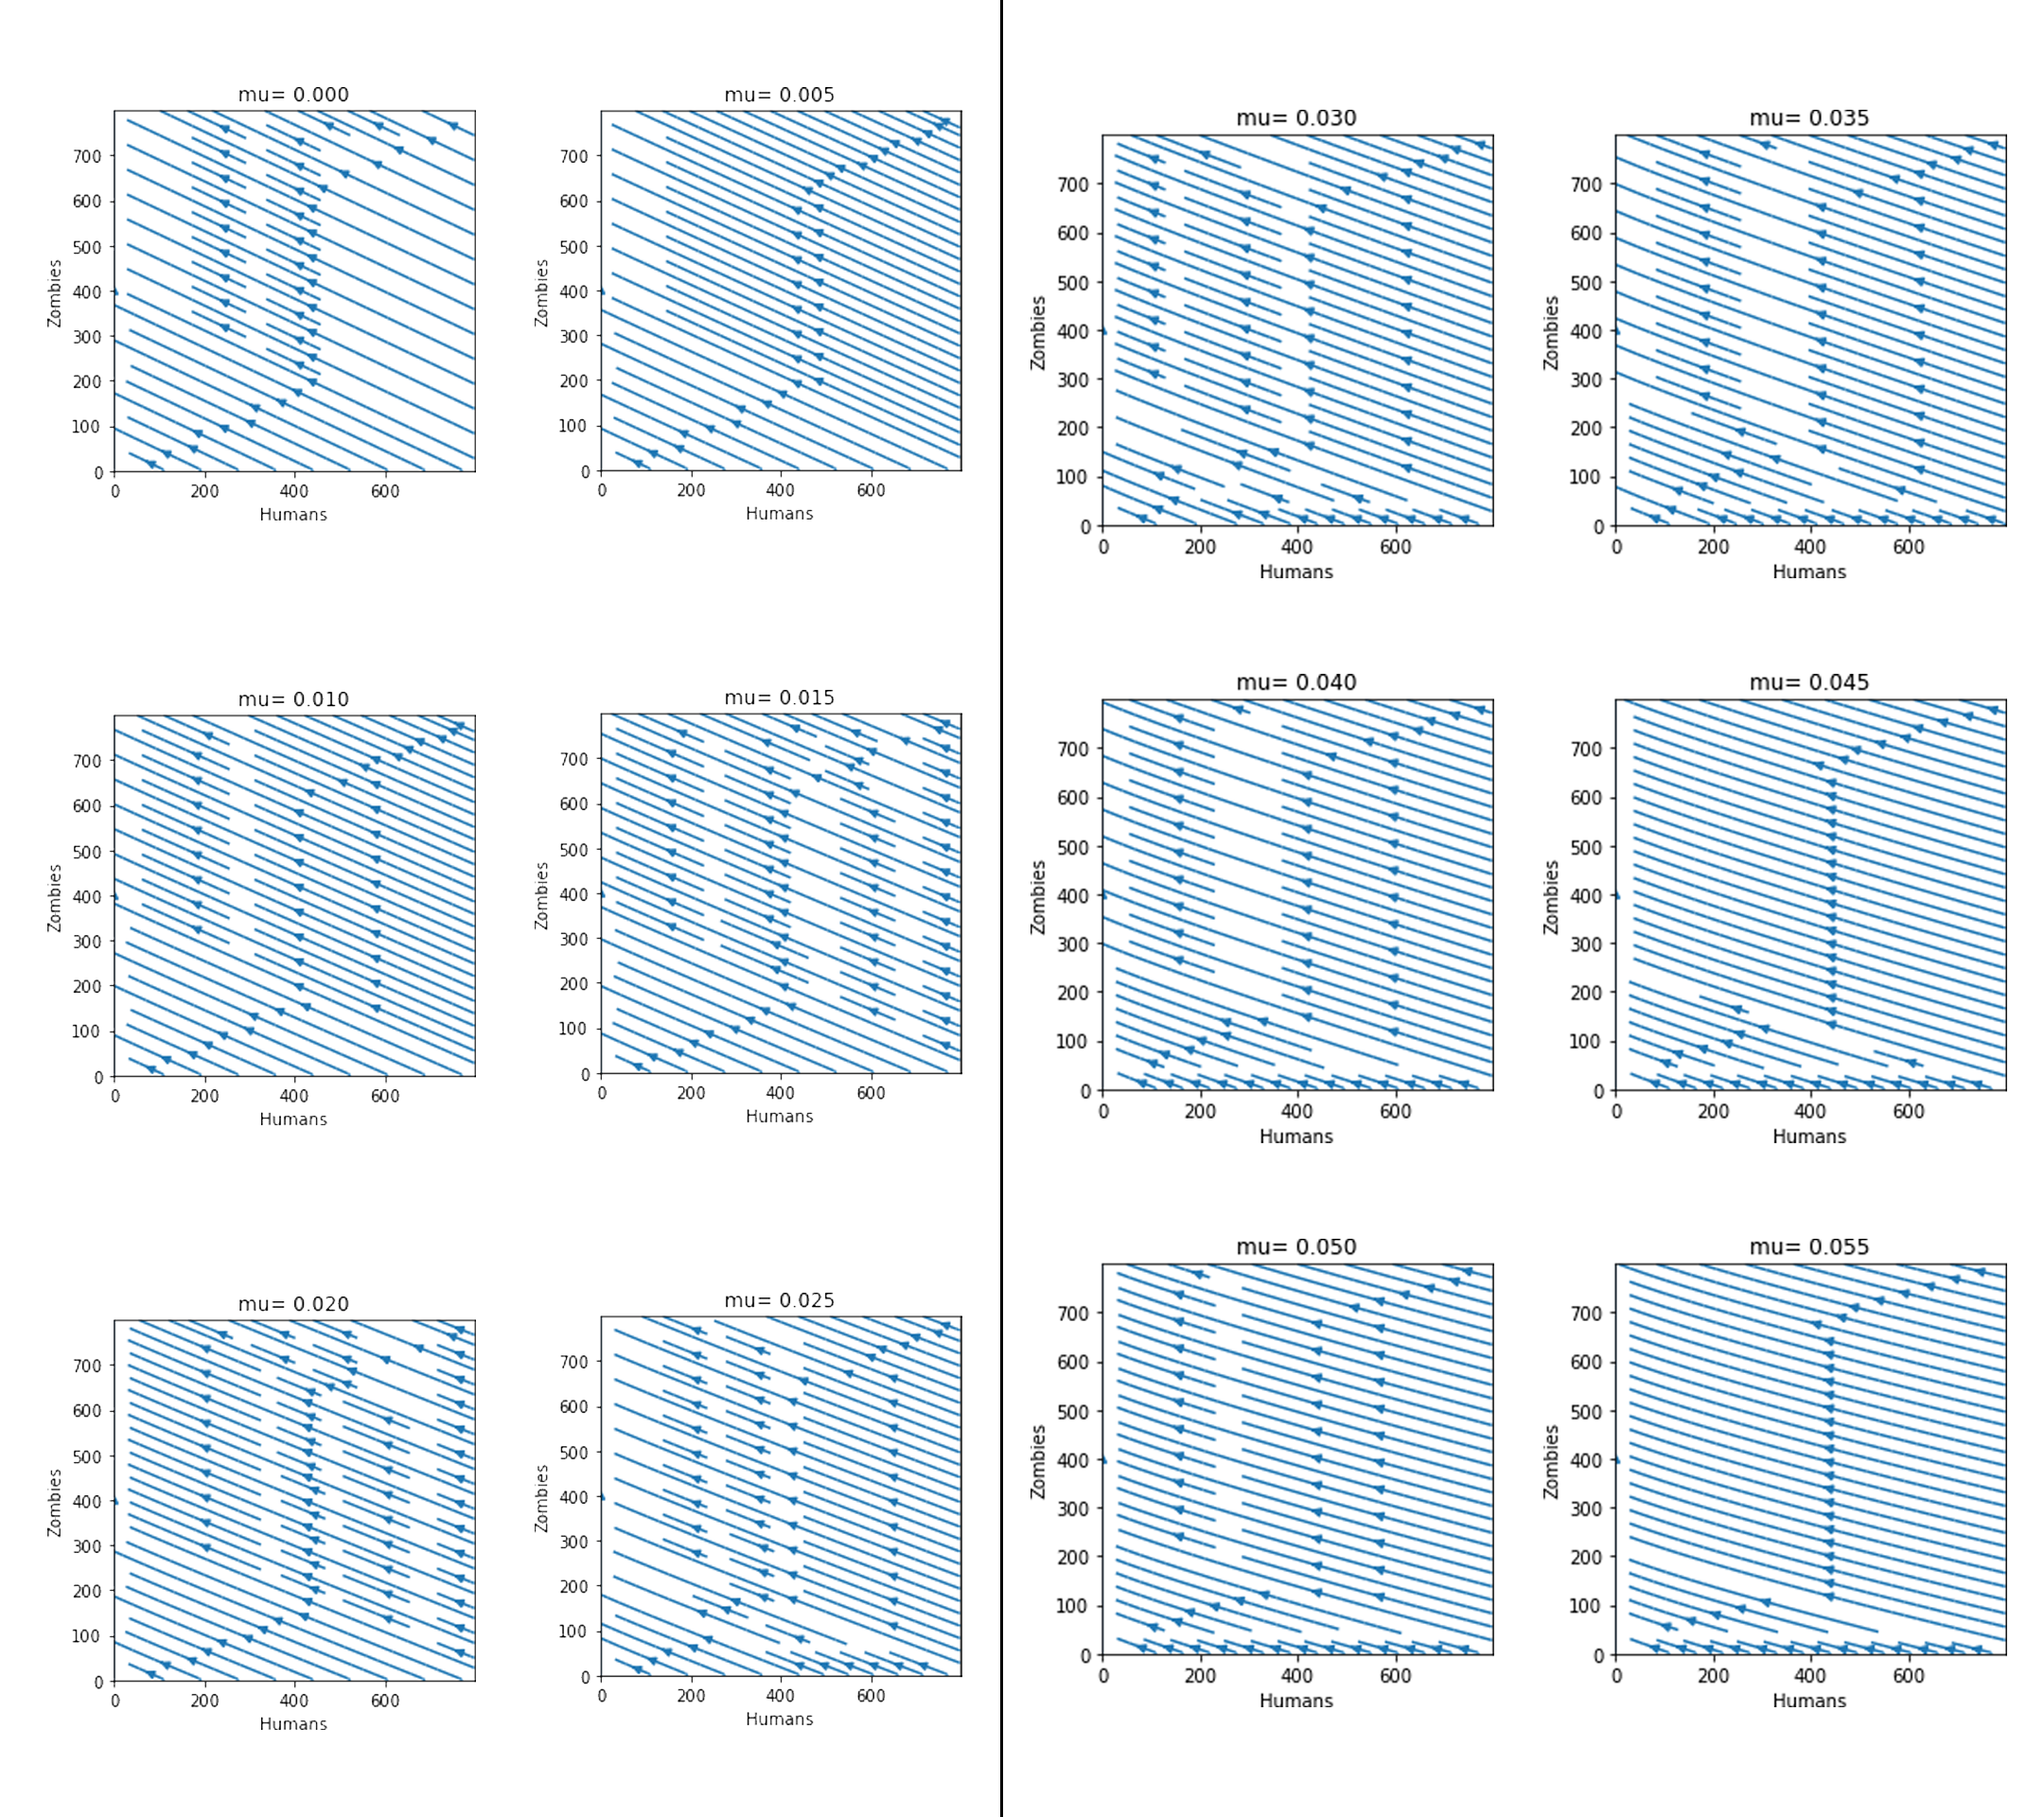
\includegraphics[scale=0.4]{finalMU_01.png}
\caption{Change of Stability, \textmu \ = 0.000 to 0.055}
\label{fig:Perturbed SZR Change of Perturbation 01}
\end{figure}

\begin{figure}[H]
\centering
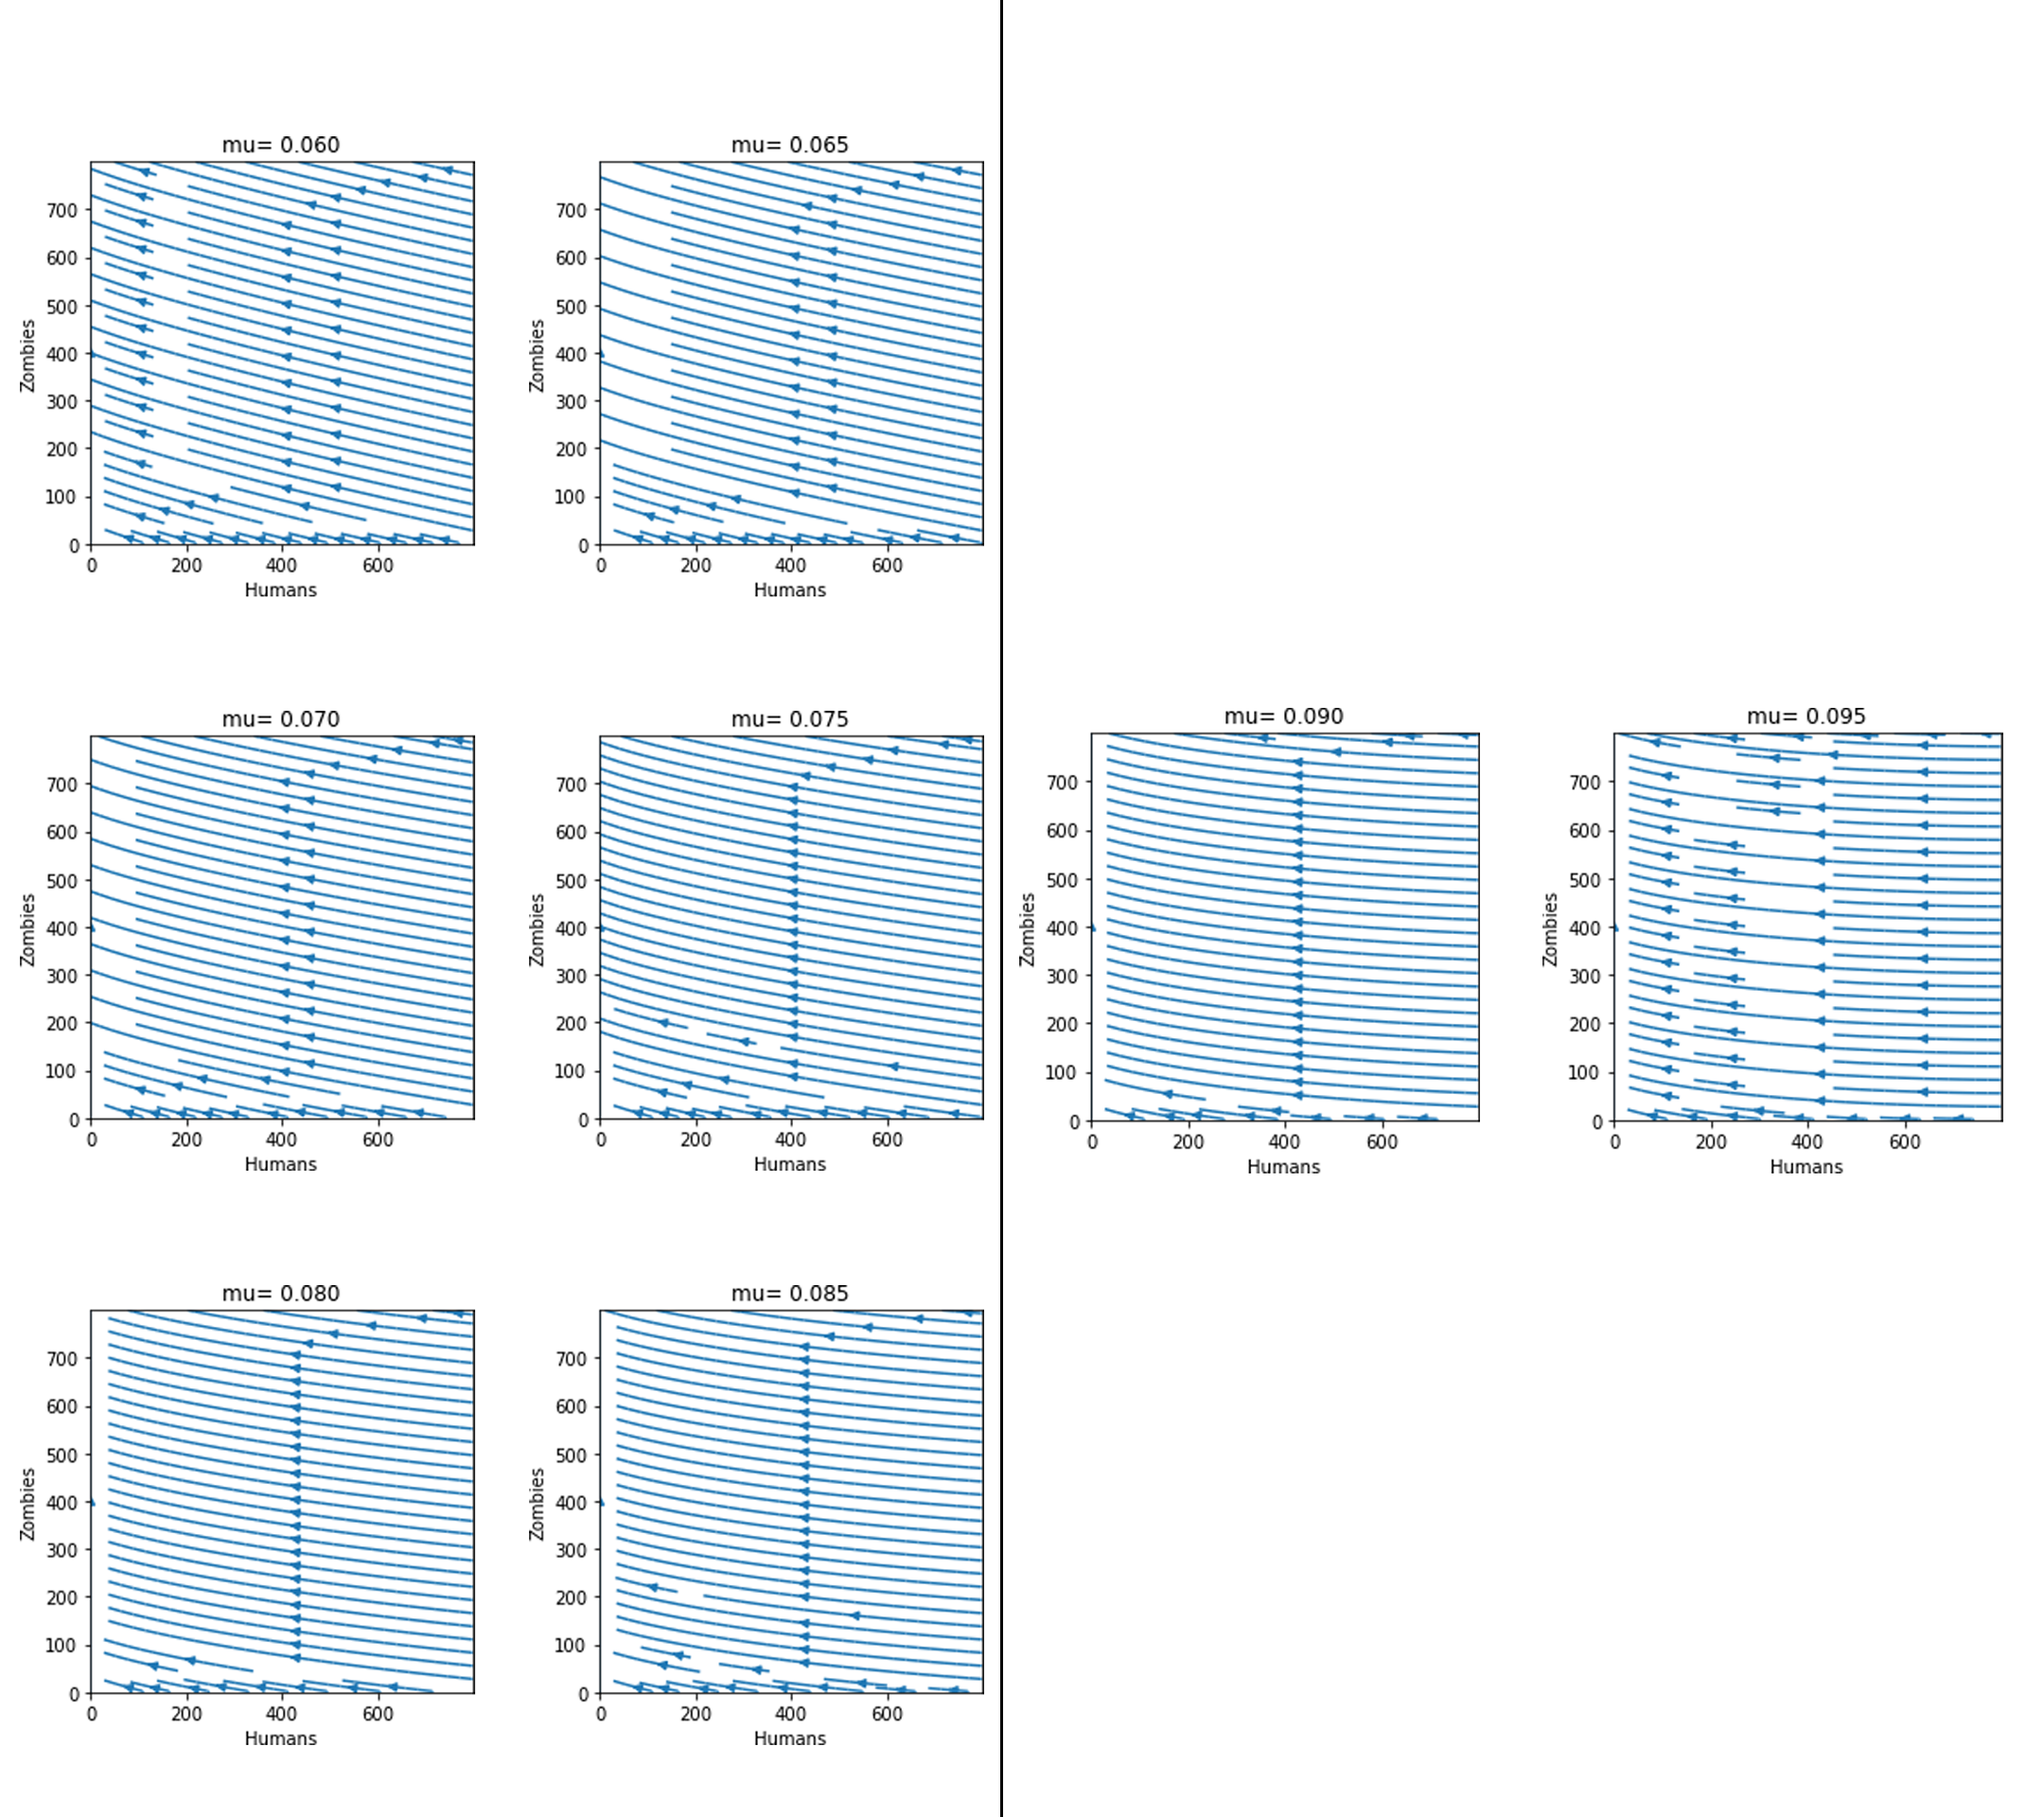
\includegraphics[scale=0.4]{finalMU_02.png}
\caption{Change of Stability, \textmu \ = 0.060 to 0.095}
\label{fig:Perturbed SZR Change of Perturbation 02}
\end{figure}

So, according to the condition stated in equation (3.5) and parameter values stated in Table (3.2), the model reaches its first stability at the value of the perturbation parameter, \textmu \ = 0.095. Starting at this perturbation value, zombie population starts to vanish gradually and the human population in the x-axis starts to increase. With each value increase of the perturbation parameter, the straight lines in the phase portraits, transform into a slightly curve lines. \\

This change in stability for the perturbed SZR model, can be visualized more conveniently with the bifurcation diagram as given below--- \\

\begin{figure}[H]
\centering
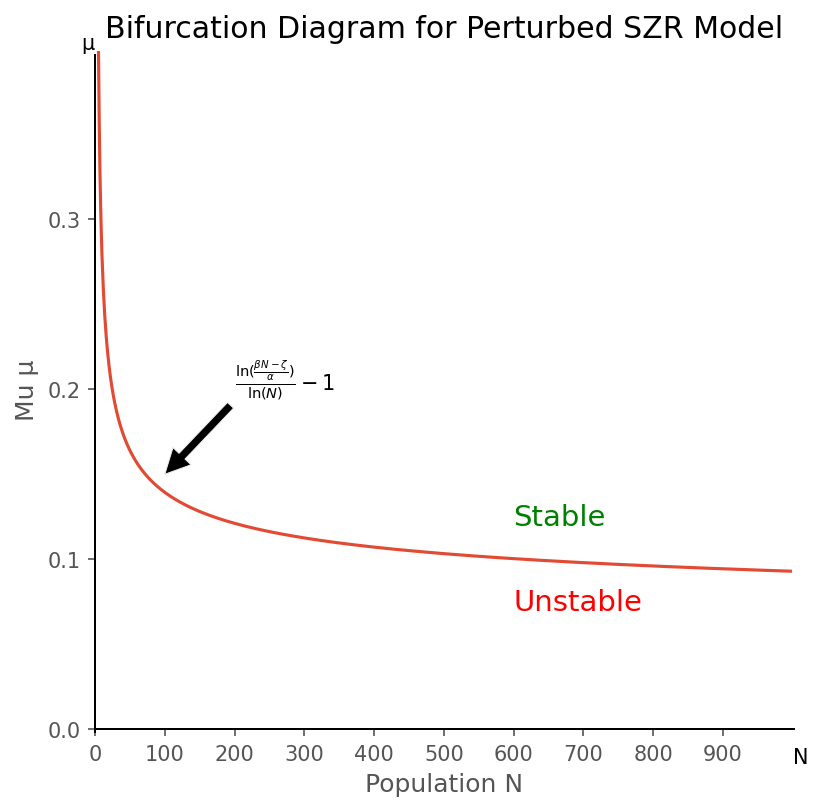
\includegraphics[scale=0.7]{PerturbedSZR_Bifurcation.png}
\caption{Bifurcation Diagram for Perturbed SZR Model}
\label{fig:Perturbed SZR Bifurcation}
\end{figure}

From the Figure 3.11, it is easily visible that the region above the curve line is stable as it satisfies the condition stated in equation (3.5). And for any value of perturbation parameter in the region below the curve line will make the model unstable. The curve line bifurcates the model, from instability to stability. 

\pagebreak
\subsection{Graphical Interface Program}

As part of writing this thesis paper, a program was created using python to develop a graphical user interface for generating phase portraits for the perturbed SZR model. This program provides the user with a simple and user friendly graphical interface to input the values of parameters \textalpha, \textbeta, \textzeta, the perturbation parameter \textmu, the population size N; and generate the phase portrait of the perturbed SZR model. It is also possible to save the generated phase portrait plot into the computer through the interactive window. So, without any more heavy coding , it is now possible to generate phase portraits and study the stability of the perturbed SZR model, just by entering the numeric parameter values inside this graphical program. \\

Some images of this interactive graphical program are given below---\\

\begin{figure}[H]
\centering
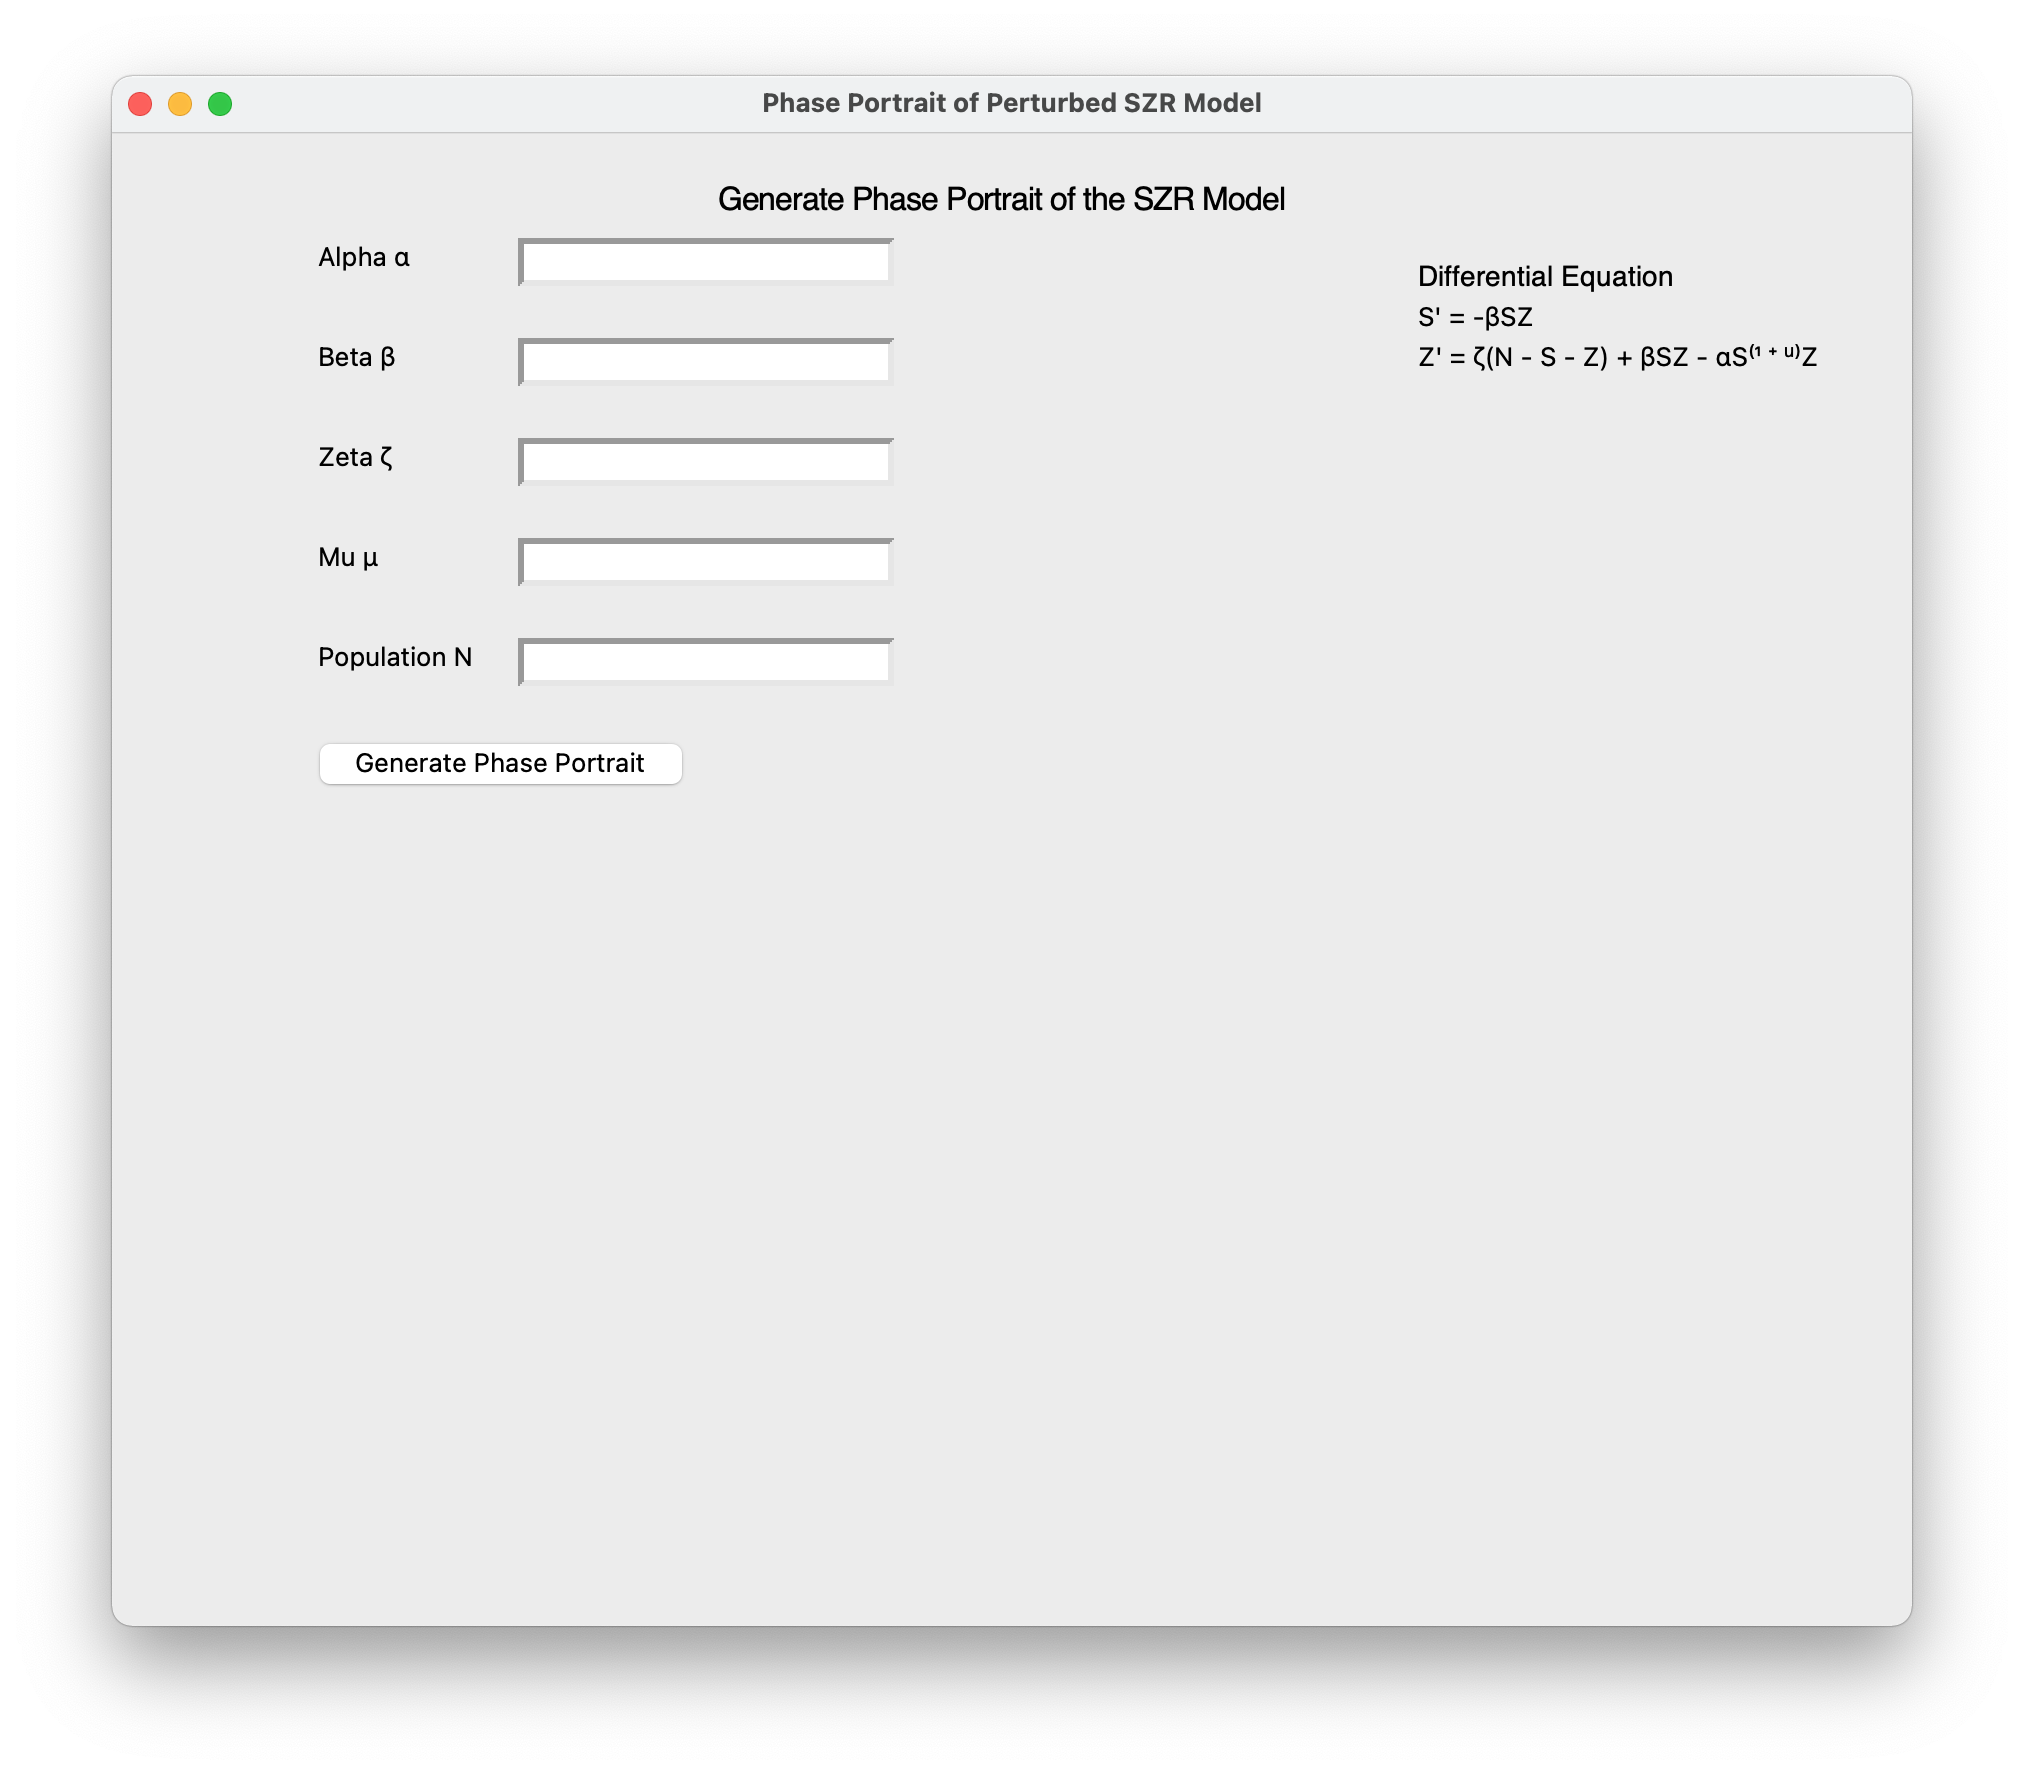
\includegraphics[scale=0.4]{PerturbedSZR_GUI.png}
\caption{GUI Program for Generating Phase Portraits, Sample 01}
\label{fig:Perturbed SZR Bifurcation GUI 01}
\end{figure}

\begin{figure}[H]
\centering
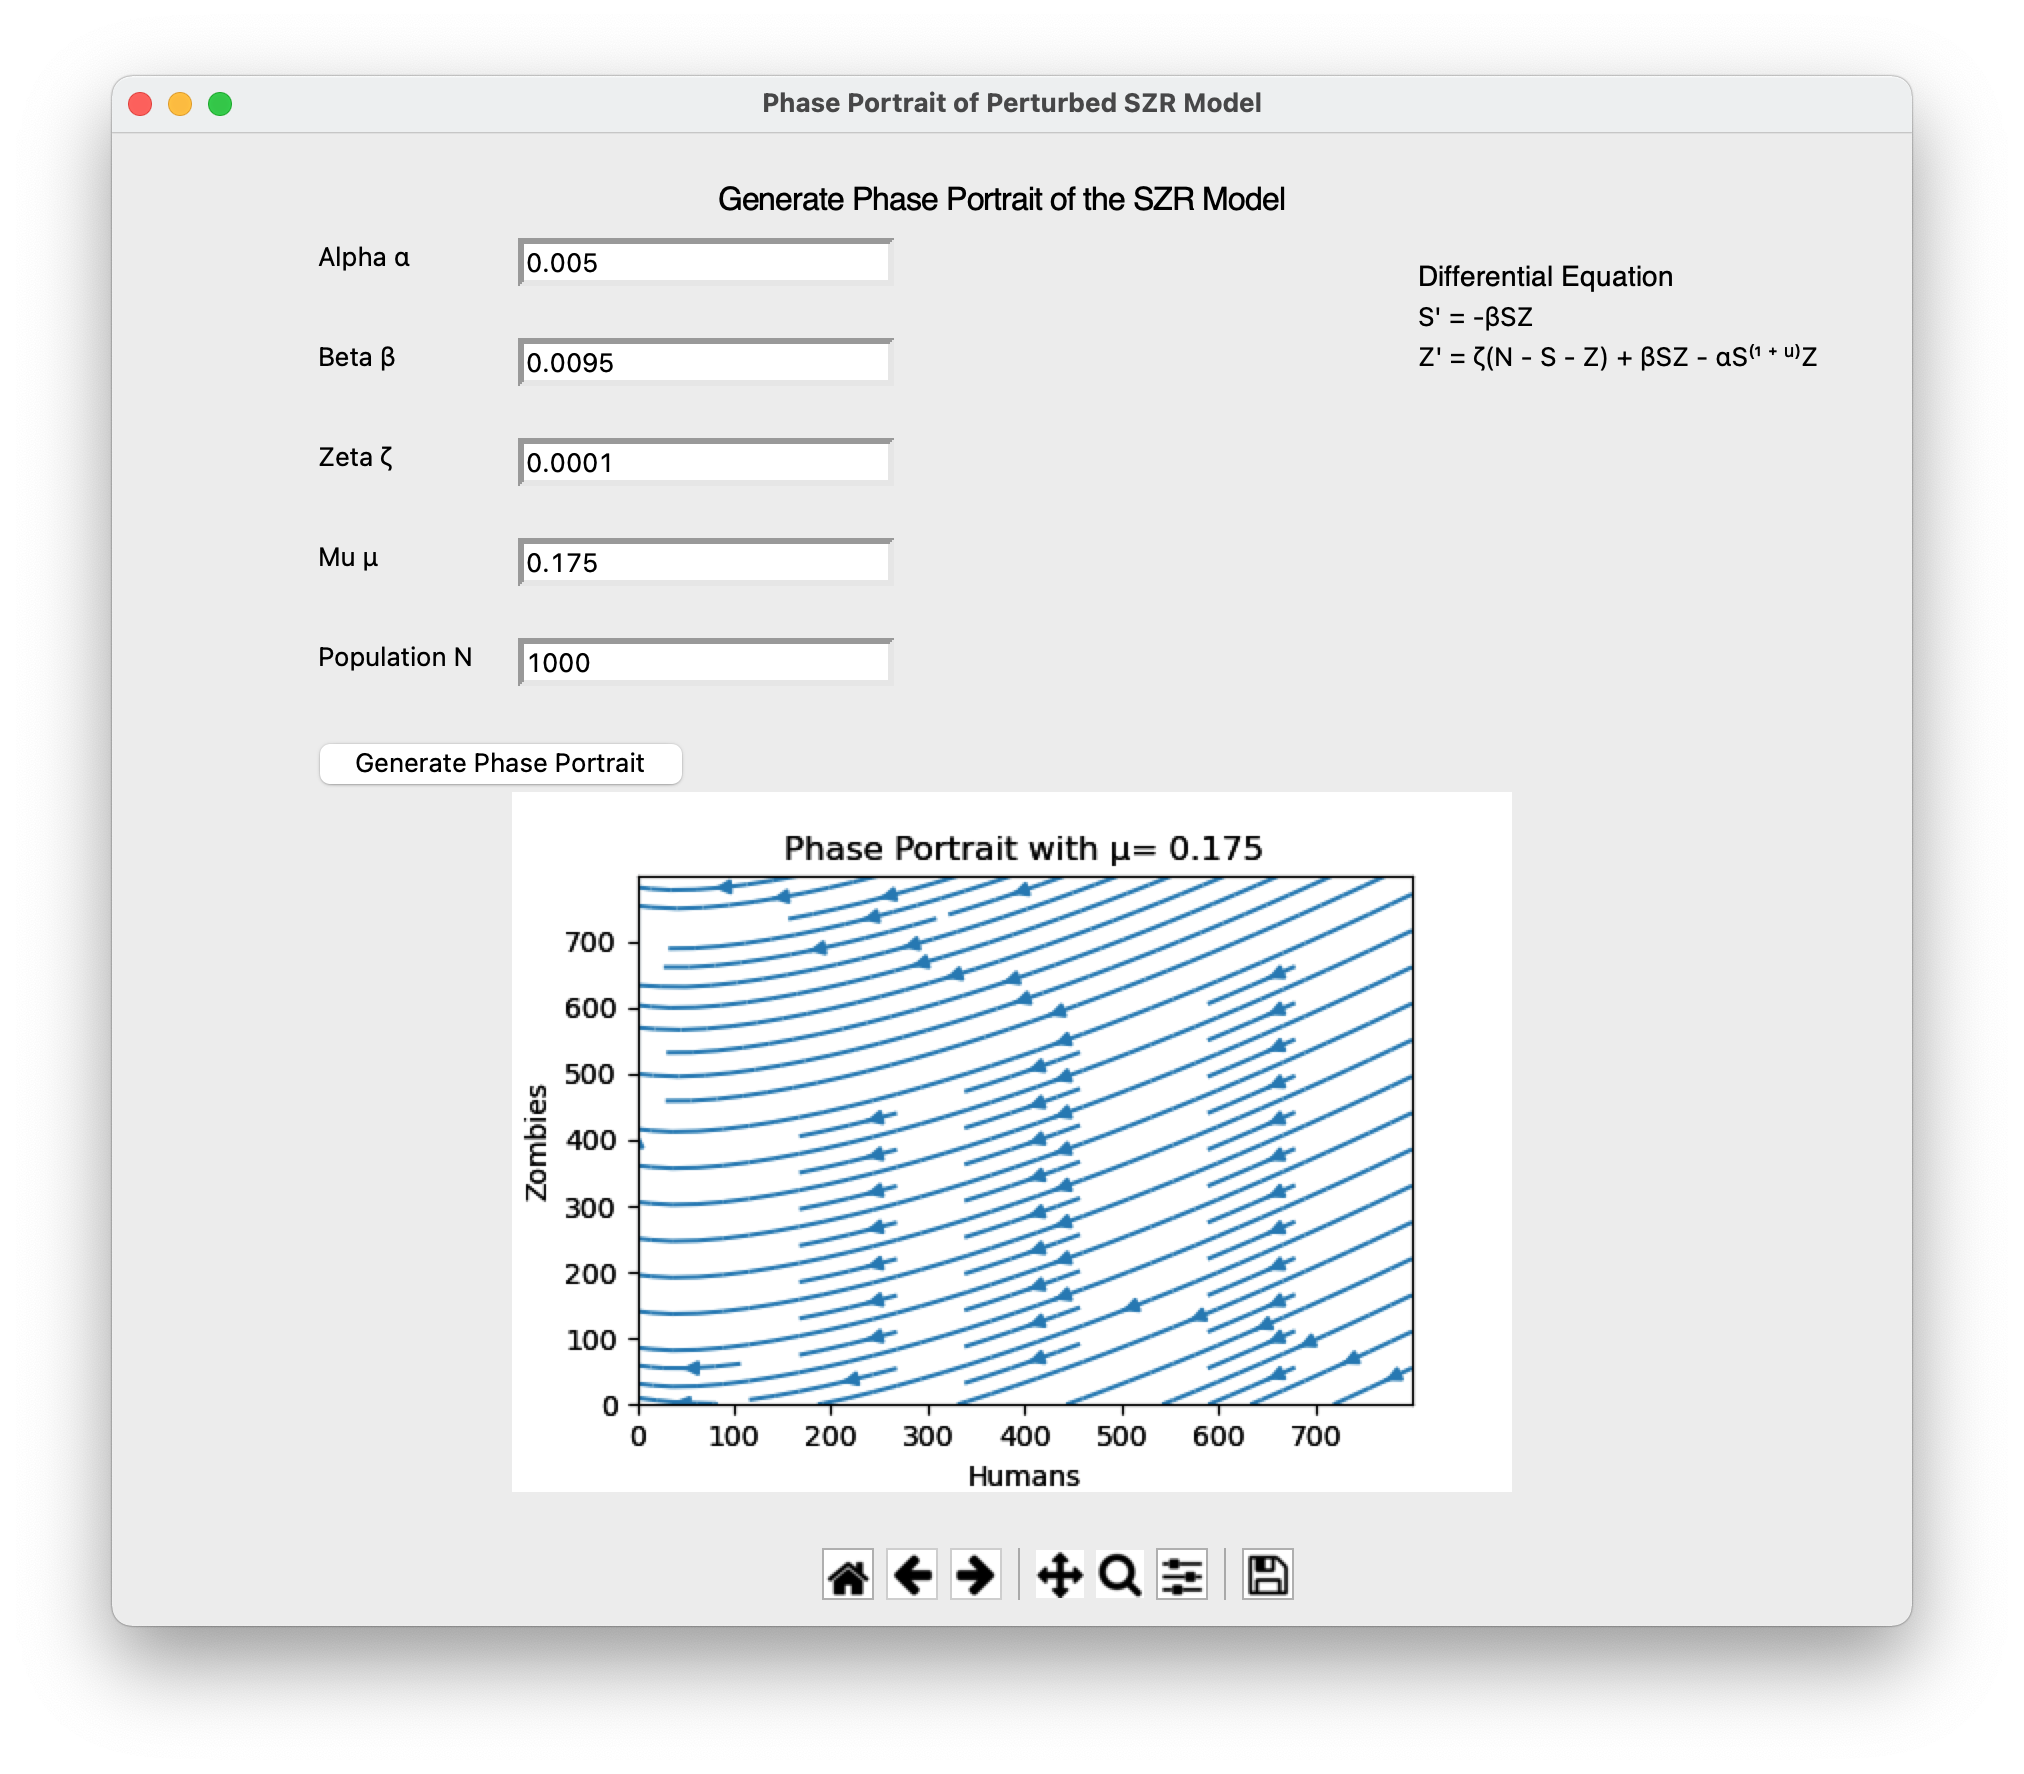
\includegraphics[scale=0.4]{PerturbedSZR_PhasePortrait_GUI.png}
\caption{GUI Program for Generating Phase Portraits, Sample 02}
\label{fig:Perturbed SZR Bifurcation GUI 02}
\end{figure}

This program was written using python and the Tkinter [47] library was used to develop the graphical user interface (GUI) for the code. This library is very fast, efficient and effective in building simple GUI applications for desktop using python. \\

The source code for this program (PerturbedSZR\_PhasePortrait\_GUI.py) is listed in the Codes section, at the end of this thesis paper. All code files are uploaded in a GitHub repository and the relevant links for downloading the source codes are also provided.  \\

\pagebreak
\subsection{Effects of Perturbation Parameter}

In order to visualize the impact of the perturbation parameter, on the model and corresponding zombie population more efficiently, two new graphs have been plotted. As for the first one, the perturbed SZR model is solved for t = 1000 days, and the population of zombies at the final 1000\textsuperscript{th} day is observed against the increase of the perturbation parameter \textmu. \\

During this calculation, the initial conditions were,\\

\noindent The total population size, N = 1000 \\
Initial susceptible population, S(0) = 800 \\
Initial zombie population, Z(0) = 200 \\
Initial removed population, R(0) = 0 \\
Number of days, t = 1000 \\

And the parameter values for \textbeta, \textalpha, \textzeta \ remain same as given on the previous Table 3.2. \\

And then the system of differential equations for the perturbed SZR model was solved using the same solve\_ivp function [23] in python. \\

The final plot looks like this as given below--- \\

\begin{figure}[H]
\centering
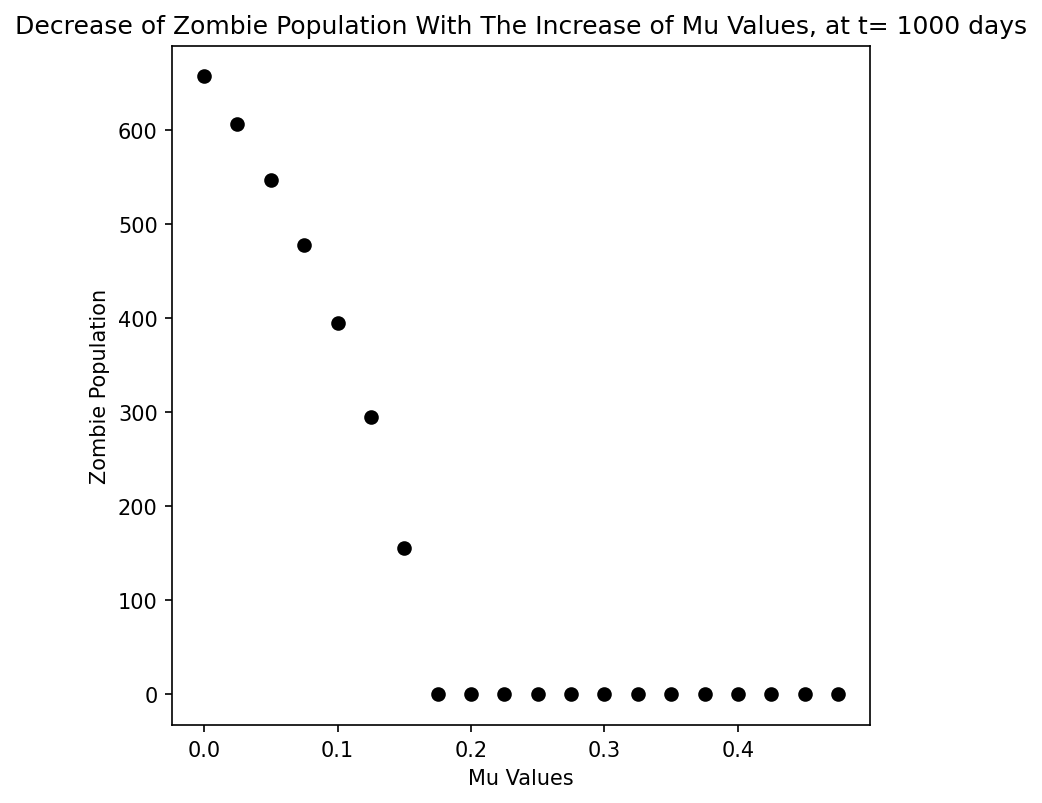
\includegraphics[scale=0.6]{ModifiedSEZQR_Zombie_Mu_Relation.png}
\caption{Perturbed SZR- Relation Between Zombie Population and Perturbation Parameter}
\label{fig:Perturbed SZR Zombie-Mu Relation 01}
\end{figure}

As can be seen from the Figure 3.14, at the final day count or at 1000\textsuperscript{th} day, the value of the zombie population decreases rapidly with the increase of perturbation parameter \textmu. The more the value of \textmu \ increases, the smaller it gets for the value of the zombie population at the 1000\textsuperscript{th} day position. And at one point, the zombie population vanishes on the 1000\textsuperscript{th} day position. \\

Also the Figure 3.15, demonstrates the whole zombie population with respect to different perturbation parameters. For different values of perturbation parameter, the zombie population is plotted in different colors, and it is visible that, with the increase of perturbation parameter values, the zombie populations decrease accordingly, and in disproportionate relation. This graph is plotted for the first 10 days only, with a step size of 0.01. So it is easier to identify the changes in the initial days. \\

\begin{figure}[H]
\centering
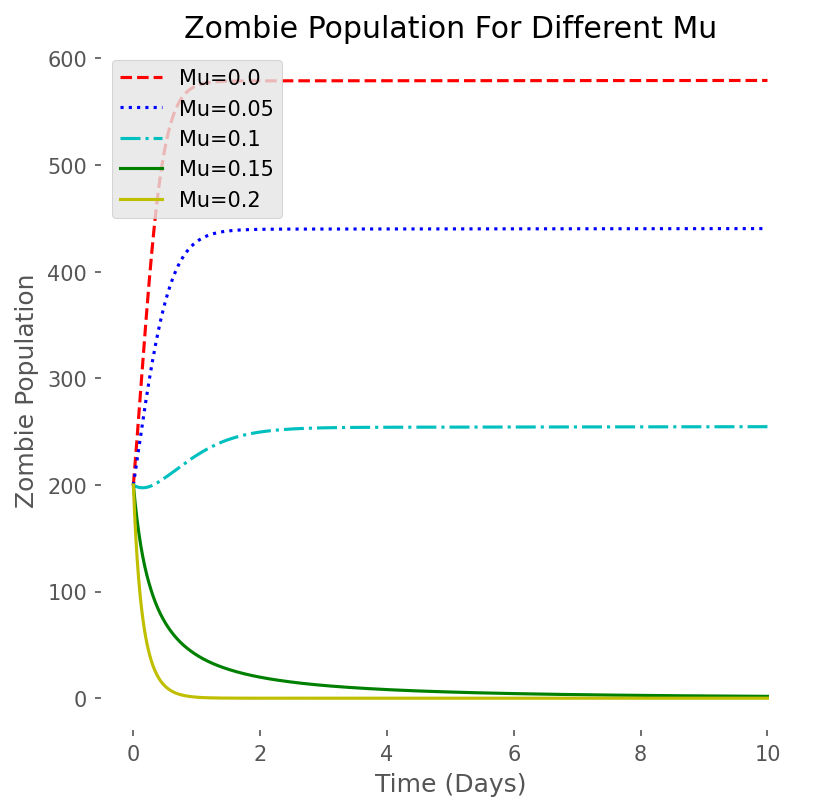
\includegraphics[scale=0.6]{PerturbedSZR_Relation_ZombieWithMu02.png}
\caption{Perturbed SZR- Zombie Population with Increasing Perturbation Parameter}
\label{fig:Perturbed SZR Zombie-Mu Relation 02}
\end{figure}

So it can be easily theorized that, the bigger the value of this perturbation parameter \textmu \ is, the faster the zombie population will disappear. The possibility to increase the value of this perturbation parameter depends on increasing the capability of human skills, equipment and methods in removing the zombies, that are available to the human population in real world. \\